\documentclass[aspectratio=169]{beamer}

% -------------------------
% Packages
% -------------------------
\usepackage[utf8]{inputenc}
\usepackage{graphicx}
\usepackage{amsmath, amssymb}
\usepackage{booktabs}
\usepackage{tcolorbox}
\usepackage{tikz}
\definecolor{questionbg}{RGB}{235, 244, 255}
\definecolor{questionframe}{RGB}{44, 95, 173}
\definecolor{plainbg}{RGB}{241, 249, 241}
\definecolor{plainframe}{RGB}{44, 122, 70}
\definecolor{notationbg}{RGB}{255, 248, 230}
\definecolor{notationframe}{RGB}{176, 118, 0}

\newtcolorbox{questionbox}{
  colback=questionbg,
  colframe=questionframe,
  boxrule=0.7pt,
  arc=1mm,
  fontupper=\small,
  left=1mm,
  right=1mm,
  top=0.4mm,
  bottom=0.4mm
}

\newtcolorbox{plainbox}{
  colback=plainbg,
  colframe=plainframe,
  boxrule=0.7pt,
  arc=1mm,
  fontupper=\small,
  left=1mm,
  right=1mm,
  top=0.4mm,
  bottom=0.4mm
}

\newtcolorbox{notationbox}{
  colback=notationbg,
  colframe=notationframe,
  boxrule=0.7pt,
  arc=1mm,
  fontupper=\small,
  left=1mm,
  right=1mm,
  top=0.4mm,
  bottom=0.4mm
}

\newcommand{\keyquestion}[1]{%
  \begin{questionbox}
  \textbf{Question:} #1
  \end{questionbox}
}

\newcommand{\plainidea}[1]{%
  \begin{plainbox}
  \textbf{Main idea:} #1
  \end{plainbox}
}

\newcommand{\notationblock}[1]{%
  \begin{notationbox}
  \textbf{Symbols used on this slide}\\
  #1
  \end{notationbox}
}

\newcommand{\exercisebreakcontent}[1]{%
  \begin{center}
  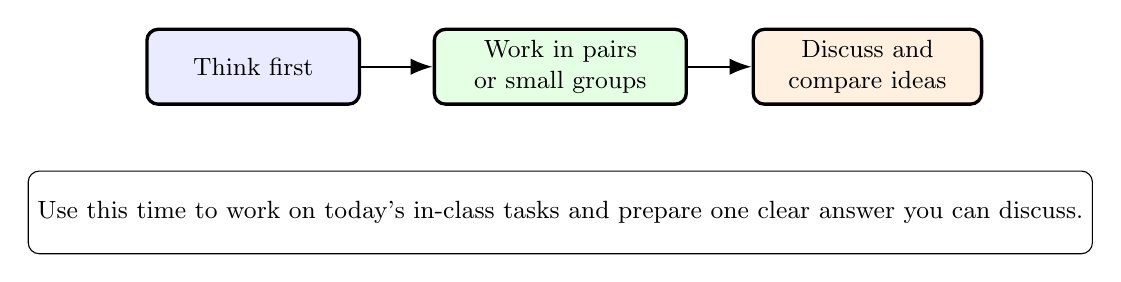
\begin{tikzpicture}[>=Latex, every node/.style={font=\small}]
    \node[draw, rounded corners, very thick, fill=blue!8, minimum width=2.7cm, minimum height=0.95cm, align=center] (think) at (-3.9,0.9) {Think first};
    \node[draw, rounded corners, very thick, fill=green!10, minimum width=3.2cm, minimum height=0.95cm, align=center] (work) at (0,0.9) {Work in pairs\\or small groups};
    \node[draw, rounded corners, very thick, fill=orange!12, minimum width=2.9cm, minimum height=0.95cm, align=center] (share) at (3.9,0.9) {Discuss and\\compare ideas};
    \draw[-{Latex[length=2.8mm]}, thick] (think) -- (work);
    \draw[-{Latex[length=2.8mm]}, thick] (work) -- (share);
    \node[draw, rounded corners, fill=white, minimum width=9.4cm, minimum height=1.05cm, align=center] at (0,-0.95) {Use this time to work on today's in-class tasks and prepare one clear answer you can discuss.};
  \end{tikzpicture}
  \end{center}
  \plainidea{#1}
}

\usepackage{hyperref}
\usetikzlibrary{positioning,arrows.meta,fit}

% -------------------------
% Theme
% -------------------------
\usetheme{Madrid}
\usecolortheme{default}
\setbeamertemplate{navigation symbols}{}

% -------------------------
% Per-slide reference footer
% -------------------------
\newcommand{\defaultdeckrefs}{AIMA4e Ch.10 pp.314--343; Poole3e Ch.16--17 pp.701--766}
\newcommand{\currentsliderefs}{\defaultdeckrefs}
\newcommand{\setslideref}[1]{\gdef\currentsliderefs{#1}}
\addtobeamertemplate{footline}{}{%
  \begin{beamercolorbox}[wd=\paperwidth,leftskip=0.4em,rightskip=0.4em,ht=2.8ex,dp=0.9ex]{author in head/foot}
    \tiny\textbf{Refs: }\currentsliderefs
  \end{beamercolorbox}
}

% -------------------------
% Metadata
% -------------------------
\title[EBU6505 B3 D3]{EBU6505 -- Reasoning and Agents\\Block 3, Day 3 -- Knowledge Graph Foundations for AI}
\author{Dr Riasat Islam}
\institute{Queen Mary University of London}
\date{}

% -------------------------
% TikZ styles
% -------------------------
\tikzset{
  flowarrow/.style={-{Latex[length=2.8mm]}, thick},
  entity/.style={draw, rounded corners, very thick, fill=blue!8, minimum width=2.2cm, minimum height=0.95cm, align=center},
  entity2/.style={draw, rounded corners, very thick, fill=green!10, minimum width=2.2cm, minimum height=0.95cm, align=center},
  relabel/.style={font=\small, fill=white, inner sep=1.5pt},
  stepbox/.style={draw, rounded corners, very thick, fill=blue!6, minimum width=2.4cm, minimum height=0.95cm, align=center},
  stepbox2/.style={draw, rounded corners, very thick, fill=green!8, minimum width=2.4cm, minimum height=0.95cm, align=center},
  note/.style={draw, rounded corners, fill=orange!12, minimum width=2.6cm, minimum height=0.9cm, align=center},
  softbox/.style={draw, rounded corners, fill=white, minimum width=2.5cm, minimum height=0.9cm, align=center}
}

\begin{document}

\setslideref{AIMA4e Ch.10 pp.314--343; Poole3e Ch.16--17 pp.701--766}
\begin{frame}
  \titlepage
\end{frame}

\begin{frame}{What have we covered so far this week?}
\begin{itemize}
  \item MDPs describe sequential decision problems.
  \item Sequential decision models use reward to compare future choices.
  \item Knowledge representation stores facts in a machine-usable form.
  \item Triples, identifiers, and schema help keep those facts clear.
\end{itemize}
\plainidea{Day 1 was about acting over time. Day 2 was about storing facts clearly. Today we connect many facts into one graph.}
\end{frame}

\begin{frame}{What are we going to cover today?}
\begin{itemize}
  \item How single triples become connected knowledge graphs
  \item How paths in a graph help answer questions
  \item Why IDs, provenance, freshness, and quality checks matter
  \item How modern AI systems retrieve small grounded pieces of a graph
\end{itemize}
\plainidea{The goal is simple: build a graph that an AI system can search, trust, and explain.}
\end{frame}

\begin{frame}{Resources}
\begin{itemize}
  \item \textit{Artificial Intelligence: Foundations of Computational Agents}, Poole and Mackworth (3rd ed.)
  \item Chapters 16 and 17 -- graph structure, knowledge graphs, and reasoning over linked facts
  \item \textit{Artificial Intelligence: A Modern Approach}, Russell and Norvig (4th ed.)
  \item Chapter 10 -- knowledge representation
\end{itemize}
\plainidea{The books give the formal view. In class, we focus on small examples that show how graph reasoning works in practice.}
\end{frame}

\begin{frame}{Learning Outcomes for Today}
By the end of this session, you should be able to:
\begin{itemize}
  \item explain how a knowledge graph differs from one isolated triple
  \item describe how graph paths support question answering and retrieval
  \item explain why identifiers, provenance, and freshness are important
  \item sketch a basic workflow for building and maintaining a small knowledge graph
\end{itemize}
\end{frame}

\begin{frame}{Warm-up Exercise}
\keyquestion{If the graph knows that Jack Ma founded Alibaba and Alibaba is in Hangzhou, what new question can it answer?}
\begin{columns}[T,onlytextwidth]
  \begin{column}{0.42\textwidth}
    \begin{itemize}
      \item Read the two connected facts.
      \item Look for a path through the graph.
      \item Say the answer in one short sentence.
    \end{itemize}
  \end{column}
  \begin{column}{0.56\textwidth}
    \begin{center}
    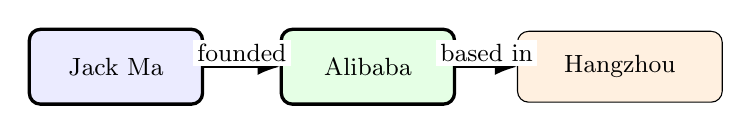
\begin{tikzpicture}[>=Latex, every node/.style={font=\small}]
      \node[entity] (ma) at (0,0) {Jack Ma};
      \node[entity2] (ali) at (3.2,0) {Alibaba};
      \node[note] (hz) at (6.4,0) {Hangzhou};
      \draw[flowarrow] (ma) -- node[relabel, above]{founded} (ali);
      \draw[flowarrow] (ali) -- node[relabel, above]{based in} (hz);
    \end{tikzpicture}
    \end{center}
  \end{column}
\end{columns}
\plainidea{A graph becomes useful when two simple facts connect and support a new question.}
\end{frame}

\begin{frame}{From One Fact to One Triple}
\keyquestion{How do we turn one sentence into a graph-friendly fact?}
\begin{columns}[T,onlytextwidth]
  \begin{column}{0.40\textwidth}
    \begin{tcolorbox}[colback=questionbg,colframe=questionframe,boxrule=0.7pt,title=Sentence]
    Alibaba is based in Hangzhou.
    \end{tcolorbox}
    \vspace{0.3em}
    \begin{itemize}
      \item Who or what is the main entity?
      \item What relation is being stated?
      \item What is the linked value or entity?
    \end{itemize}
  \end{column}
  \begin{column}{0.56\textwidth}
    \begin{center}
    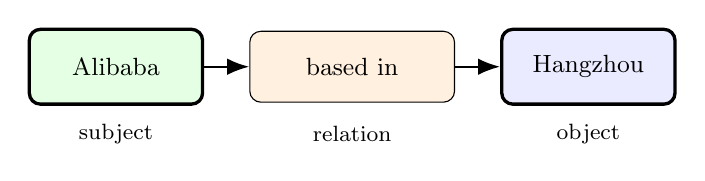
\begin{tikzpicture}[>=Latex, every node/.style={font=\small}]
      \node[entity2] (s) at (0,0) {Alibaba};
      \node[note] (p) at (3.0,0) {based in};
      \node[entity] (o) at (6.0,0) {Hangzhou};
      \draw[flowarrow] (s) -- (p);
      \draw[flowarrow] (p) -- (o);
      \node[font=\footnotesize] at (0,-0.85) {subject};
      \node[font=\footnotesize] at (3.0,-0.85) {relation};
      \node[font=\footnotesize] at (6.0,-0.85) {object};
    \end{tikzpicture}
    \end{center}
  \end{column}
\end{columns}
\plainidea{A triple keeps one fact short, explicit, and easy for a machine to reuse later.}
\end{frame}

\begin{frame}{From Many Triples to One Graph}
\keyquestion{What changes when several triples share the same entities?}
\begin{center}
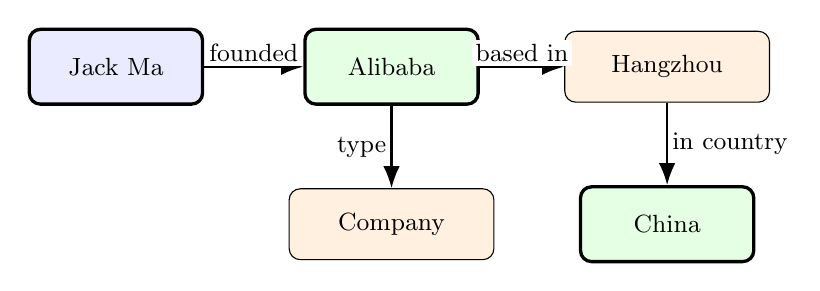
\begin{tikzpicture}[>=Latex, every node/.style={font=\small}]
  \node[entity] (ma) at (0,1.2) {Jack Ma};
  \node[entity2] (ali) at (3.5,1.2) {Alibaba};
  \node[note] (hz) at (7,1.2) {Hangzhou};
  \node[entity2] (china) at (7,-0.8) {China};
  \node[note] (company) at (3.5,-0.8) {Company};
  \draw[flowarrow] (ma) -- node[relabel, above]{founded} (ali);
  \draw[flowarrow] (ali) -- node[relabel, above]{based in} (hz);
  \draw[flowarrow] (hz) -- node[relabel, right]{in country} (china);
  \draw[flowarrow] (ali) -- node[relabel, left]{type} (company);
\end{tikzpicture}
\end{center}
\plainidea{A knowledge graph is not just one fact. It is a network of facts that share entities and relations.}
\end{frame}

\begin{frame}{Entities, Relations, and Attributes}
\keyquestion{What kinds of things do we usually store in a knowledge graph?}
\begin{columns}[T,onlytextwidth]
  \begin{column}{0.34\textwidth}
    \begin{tcolorbox}[colback=questionbg,colframe=questionframe,boxrule=0.7pt,title=Three core parts]
    \textbf{Entity}: main thing\\[0.3em]
    \textbf{Relation}: named link\\[0.3em]
    \textbf{Attribute}: property value
    \end{tcolorbox}
  \end{column}
  \begin{column}{0.62\textwidth}
    \begin{center}
    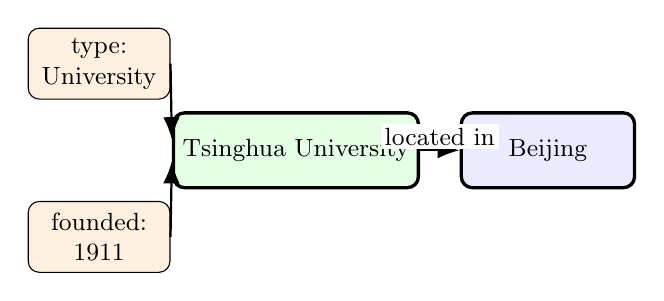
\begin{tikzpicture}[>=Latex, every node/.style={font=\small}]
      \node[entity2, minimum width=3.0cm] (uni) at (2.5,0.1) {Tsinghua University};
      \node[entity, minimum width=2.2cm] (city) at (5.7,0.1) {Beijing};
      \node[note, minimum width=1.8cm] (type) at (0.0,1.2) {type:\\ University};
      \node[note, minimum width=1.8cm] (year) at (0.0,-1.0) {founded:\\ 1911};
      \draw[flowarrow] (uni) -- node[relabel, above]{located in} (city);
      \draw[flowarrow] (type.east) -- ([yshift=4pt]uni.west);
      \draw[flowarrow] (year.east) -- ([yshift=-4pt]uni.west);
    \end{tikzpicture}
    \end{center}
  \end{column}
\end{columns}
\plainidea{Entities are the main nodes. Relations connect entities. Attributes add small details.}
\end{frame}

\begin{frame}{Why IDs Matter}
\keyquestion{Why is the name alone often not enough for a graph?}
\begin{columns}[T,onlytextwidth]
  \begin{column}{0.48\textwidth}
    \begin{tcolorbox}[colback=questionbg,colframe=questionframe,boxrule=0.7pt,title=Name only]
    ``Apple'' can mean:
    \begin{itemize}
      \item the company
      \item the fruit
    \end{itemize}
    \end{tcolorbox}
  \end{column}
  \begin{column}{0.48\textwidth}
    \begin{center}
    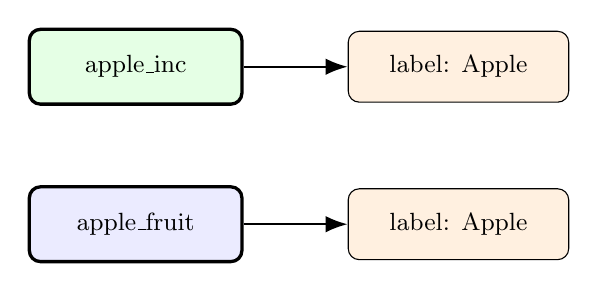
\begin{tikzpicture}[>=Latex, every node/.style={font=\small}]
      \node[entity2, minimum width=2.7cm] (c) at (0,1.0) {apple\_inc};
      \node[entity, minimum width=2.7cm] (f) at (0,-1.0) {apple\_fruit};
      \node[note, minimum width=2.8cm] (cn) at (4.1,1.0) {label: Apple};
      \node[note, minimum width=2.8cm] (fn) at (4.1,-1.0) {label: Apple};
      \draw[flowarrow] (c) -- (cn);
      \draw[flowarrow] (f) -- (fn);
    \end{tikzpicture}
    \end{center}
  \end{column}
\end{columns}
\plainidea{A good graph gives each entity a stable ID, even when two entities share the same name.}
\end{frame}

\begin{frame}{Relation Design Must Be Precise}
\keyquestion{Why are vague relation names bad for retrieval and reasoning?}
\begin{columns}[T,onlytextwidth]
  \begin{column}{0.48\textwidth}
    \begin{tcolorbox}[colback=red!6,colframe=red!60!black,boxrule=0.7pt,title=Too vague]
    \begin{itemize}
      \item related to
      \item connected to
      \item associated with
    \end{itemize}
    \end{tcolorbox}
  \end{column}
  \begin{column}{0.48\textwidth}
    \begin{tcolorbox}[colback=green!6,colframe=green!50!black,boxrule=0.7pt,title=Clearer]
    \begin{itemize}
      \item founded
      \item based in
      \item taught by
    \end{itemize}
    \end{tcolorbox}
  \end{column}
\end{columns}
\begin{center}
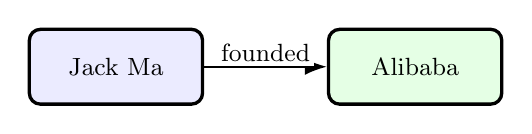
\begin{tikzpicture}[>=Latex, every node/.style={font=\small}]
  \node[entity] (s1) at (0,0) {Jack Ma};
  \node[entity2] (o1) at (3.8,0) {Alibaba};
  \draw[flowarrow] (s1) -- node[relabel, above]{founded} (o1);
\end{tikzpicture}
\end{center}
\plainidea{If relation names are clear, the system can retrieve the right path and explain the answer more easily.}
\end{frame}

\begin{frame}{Pattern Versus Real Facts}
\keyquestion{What is the difference between a graph pattern and one actual set of facts?}
\begin{columns}[T,onlytextwidth]
  \begin{column}{0.48\textwidth}
    \begin{tcolorbox}[colback=questionbg,colframe=questionframe,boxrule=0.7pt,title=Schema idea]
    Person -- founded -- Company -- based in -- City
    \end{tcolorbox}
    \begin{center}
    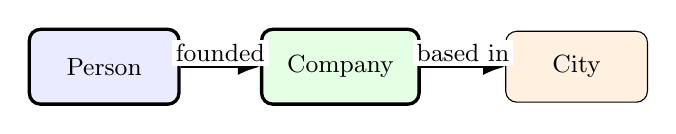
\begin{tikzpicture}[>=Latex, every node/.style={font=\small}]
      \node[entity, minimum width=1.9cm] (p) at (0,0) {Person};
      \node[entity2, minimum width=2.0cm] (c) at (3.0,0) {Company};
      \node[note, minimum width=1.8cm] (city) at (6.0,0) {City};
      \draw[flowarrow] (p) -- node[relabel, above]{founded} (c);
      \draw[flowarrow] (c) -- node[relabel, above]{based in} (city);
    \end{tikzpicture}
    \end{center}
  \end{column}
  \begin{column}{0.48\textwidth}
    \begin{tcolorbox}[colback=plainbg,colframe=plainframe,boxrule=0.7pt,title=Instance idea]
    Jack Ma -- founded -- Alibaba -- based in -- Hangzhou
    \end{tcolorbox}
    \begin{center}
    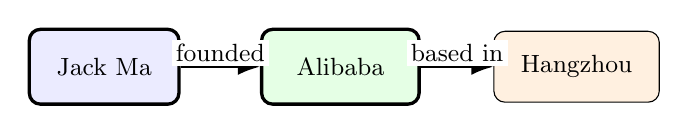
\begin{tikzpicture}[>=Latex, every node/.style={font=\small}]
      \node[entity, minimum width=1.9cm] (p) at (0,0) {Jack Ma};
      \node[entity2, minimum width=2.0cm] (c) at (3.0,0) {Alibaba};
      \node[note, minimum width=2.1cm] (city) at (6.0,0) {Hangzhou};
      \draw[flowarrow] (p) -- node[relabel, above]{founded} (c);
      \draw[flowarrow] (c) -- node[relabel, above]{based in} (city);
    \end{tikzpicture}
    \end{center}
  \end{column}
\end{columns}
\plainidea{The schema gives the pattern. The instance graph fills that pattern with real entities and real facts.}
\end{frame}

\begin{frame}{A Graph Path Can Be the Answer}
\keyquestion{How can the graph answer the question ``Who founded Alibaba?''}
\begin{center}
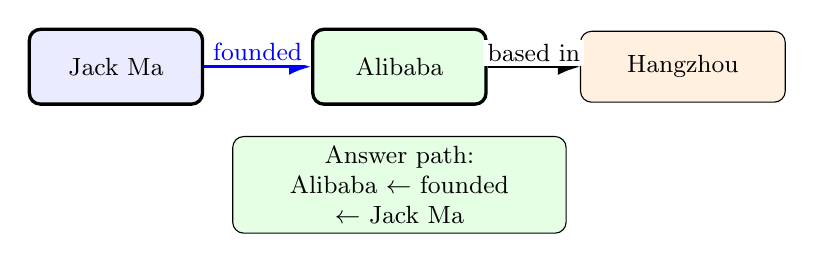
\begin{tikzpicture}[>=Latex, every node/.style={font=\small}]
  \node[entity] (ma) at (0,0.3) {Jack Ma};
  \node[entity2] (ali) at (3.6,0.3) {Alibaba};
  \node[note] (hz) at (7.2,0.3) {Hangzhou};
  \draw[flowarrow, very thick, blue] (ma) -- node[relabel, above]{founded} (ali);
  \draw[flowarrow] (ali) -- node[relabel, above]{based in} (hz);
  \node[draw, rounded corners, fill=green!10, text width=4.0cm, minimum height=0.95cm, align=center] at (3.6,-1.2) {Answer path:\\ Alibaba $\leftarrow$ founded $\leftarrow$ Jack Ma};
\end{tikzpicture}
\end{center}
\plainidea{The system can follow the right graph edge instead of scanning unrelated text.}
\end{frame}

\begin{frame}{Multi-Hop Reasoning}
\keyquestion{How can two connected edges answer a harder question?}
\begin{columns}[T,onlytextwidth]
  \begin{column}{0.44\textwidth}
    \begin{tcolorbox}[colback=questionbg,colframe=questionframe,boxrule=0.7pt,title=Question]
    Which city is the company founded by Jack Ma based in?
    \end{tcolorbox}
    \begin{itemize}
      \item Step 1: find the company founded by Jack Ma.
      \item Step 2: follow the next edge from that company.
    \end{itemize}
  \end{column}
  \begin{column}{0.54\textwidth}
    \begin{center}
    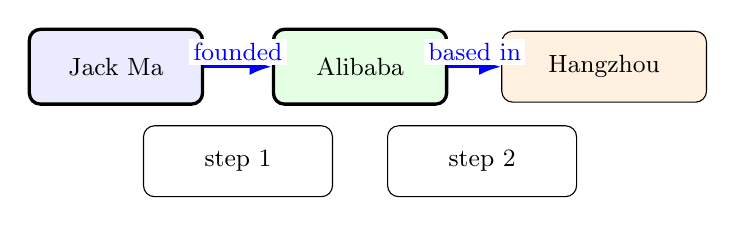
\begin{tikzpicture}[>=Latex, every node/.style={font=\small}]
      \node[entity] (ma) at (0,0) {Jack Ma};
      \node[entity2] (ali) at (3.1,0) {Alibaba};
      \node[note] (hz) at (6.2,0) {Hangzhou};
      \draw[flowarrow, very thick, blue] (ma) -- node[relabel, above]{founded} (ali);
      \draw[flowarrow, very thick, blue] (ali) -- node[relabel, above]{based in} (hz);
      \node[softbox, minimum width=2.4cm] at (1.55,-1.2) {step 1};
      \node[softbox, minimum width=2.4cm] at (4.65,-1.2) {step 2};
    \end{tikzpicture}
    \end{center}
  \end{column}
\end{columns}
\plainidea{Multi-hop reasoning means following more than one edge to reach the answer.}
\end{frame}

\begin{frame}{Neighborhood Retrieval for AI}
\keyquestion{When a user asks one question, should the system read the whole graph?}
\begin{columns}[T,onlytextwidth]
  \begin{column}{0.40\textwidth}
    \begin{tcolorbox}[colback=questionbg,colframe=questionframe,boxrule=0.7pt,title=User query]
    Where is Alibaba based?
    \end{tcolorbox}
    \begin{itemize}
      \item Link the query to the entity Alibaba.
      \item Retrieve only the nearby facts.
      \item Highlight the edge that answers the question.
    \end{itemize}
  \end{column}
  \begin{column}{0.56\textwidth}
    \begin{center}
    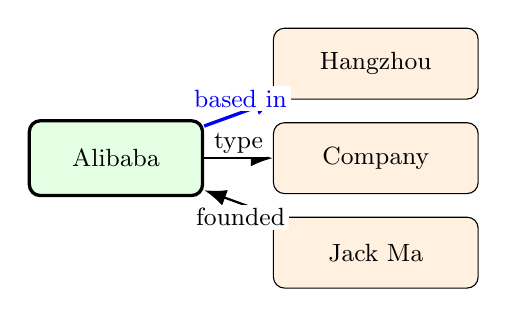
\begin{tikzpicture}[>=Latex, every node/.style={font=\small}]
      \node[entity2] (ali) at (0,0) {Alibaba};
      \node[note] (hz) at (3.3,1.2) {Hangzhou};
      \node[note] (type) at (3.3,0) {Company};
      \node[note] (founder) at (3.3,-1.2) {Jack Ma};
      \draw[flowarrow, very thick, blue] (ali) -- node[relabel, above]{based in} (hz);
      \draw[flowarrow] (ali) -- node[relabel, above]{type} (type);
      \draw[flowarrow] (founder) -- node[relabel, below]{founded} (ali);
    \end{tikzpicture}
    \end{center}
  \end{column}
\end{columns}
\plainidea{Good retrieval starts from the right entity and keeps only the useful neighborhood.}
\end{frame}

\begin{frame}{Common Data-Quality Problems}
\keyquestion{What can go wrong if a graph is badly maintained?}
\begin{columns}[T,onlytextwidth]
  \begin{column}{0.48\textwidth}
    \begin{tcolorbox}[colback=red!6,colframe=red!60!black,boxrule=0.7pt,title=Wrong fact]
    Example: wrong city stored
    \end{tcolorbox}
    \begin{tcolorbox}[colback=orange!10,colframe=orange!70!black,boxrule=0.7pt,title=Missing link]
    Example: headquarters link missing
    \end{tcolorbox}
  \end{column}
  \begin{column}{0.48\textwidth}
    \begin{tcolorbox}[colback=blue!6,colframe=blue!60!black,boxrule=0.7pt,title=Duplicate entity]
    Example: one person stored twice
    \end{tcolorbox}
    \begin{tcolorbox}[colback=green!6,colframe=green!50!black,boxrule=0.7pt,title=Old fact]
    Example: location changed, graph not updated
    \end{tcolorbox}
  \end{column}
\end{columns}
\plainidea{A graph is useful only when its facts are correct, complete enough, and up to date.}
\end{frame}

\begin{frame}{Why Provenance Matters}
\keyquestion{How do we know where one graph fact came from?}
\begin{center}
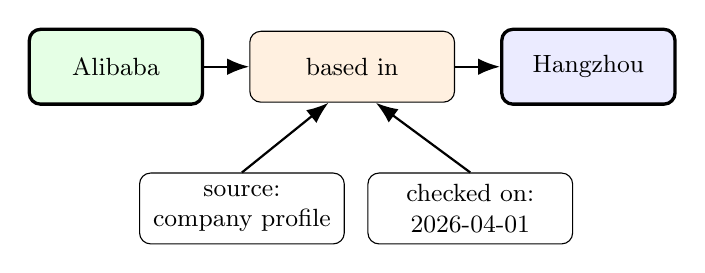
\begin{tikzpicture}[>=Latex, every node/.style={font=\small}]
  \node[entity2] (ali) at (0,0) {Alibaba};
  \node[note] (rel) at (3.0,0) {based in};
  \node[entity] (hz) at (6.0,0) {Hangzhou};
  \draw[flowarrow] (ali) -- (rel);
  \draw[flowarrow] (rel) -- (hz);
  \node[softbox, minimum width=2.6cm] (src) at (1.6,-1.8) {source:\\ company profile};
  \node[softbox, minimum width=2.6cm] (date) at (4.5,-1.8) {checked on:\\ 2026-04-01};
  \draw[flowarrow] (src.north) -- ([xshift=-0.3cm]rel.south);
  \draw[flowarrow] (date.north) -- ([xshift=0.3cm]rel.south);
\end{tikzpicture}
\end{center}
\plainidea{Provenance tells us the source and date of a fact, so we can trust it, check it, and explain it.}
\end{frame}

\begin{frame}{Freshness Matters Too}
\keyquestion{Why is a correct old fact still a problem?}
\begin{center}
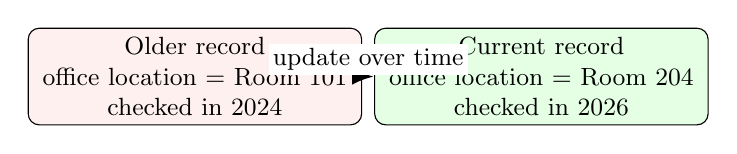
\begin{tikzpicture}[>=Latex, every node/.style={font=\small}]
  \node[draw, rounded corners, fill=red!6, text width=4.0cm, minimum height=1.2cm, align=center] (old) at (1.7,0) {Older record\\ office location = Room 101\\ checked in 2024};
  \node[draw, rounded corners, fill=green!10, text width=4.0cm, minimum height=1.2cm, align=center] (new) at (6.1,0) {Current record\\ office location = Room 204\\ checked in 2026};
  \draw[flowarrow, very thick] (old) -- node[relabel, above]{update over time} (new);
\end{tikzpicture}
\end{center}
\plainidea{A graph should not just store facts. It should also know when those facts were last checked.}
\end{frame}

\begin{frame}{Entity Resolution}
\keyquestion{How do we avoid storing the same real entity more than once?}
\begin{columns}[T,onlytextwidth]
  \begin{column}{0.44\textwidth}
    \begin{center}
    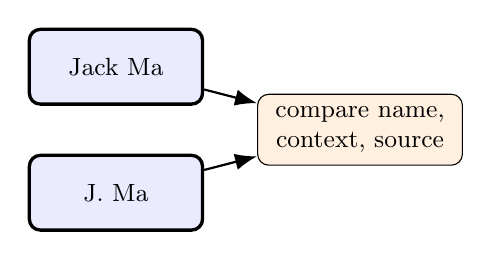
\begin{tikzpicture}[>=Latex, every node/.style={font=\small}]
      \node[entity] (a) at (0,0.8) {Jack Ma};
      \node[entity] (b) at (0,-0.8) {J. Ma};
      \node[note] (check) at (3.1,0) {compare name,\\ context, source};
      \draw[flowarrow] (a) -- (check);
      \draw[flowarrow] (b) -- (check);
    \end{tikzpicture}
    \end{center}
  \end{column}
  \begin{column}{0.52\textwidth}
    \begin{center}
    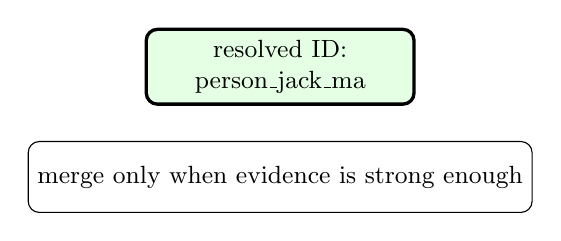
\begin{tikzpicture}[>=Latex, every node/.style={font=\small}]
      \node[entity2, minimum width=3.4cm] (m) at (0,0) {resolved ID:\\ person\_jack\_ma};
      \node[softbox, minimum width=3.8cm] at (0,-1.4) {merge only when evidence is strong enough};
    \end{tikzpicture}
    \end{center}
  \end{column}
\end{columns}
\plainidea{Entity resolution is the process of deciding whether two records refer to the same real thing.}
\end{frame}

\begin{frame}{How to Build a Small Practical KG}
\keyquestion{What are the main steps from raw text to a usable graph?}
\begin{center}
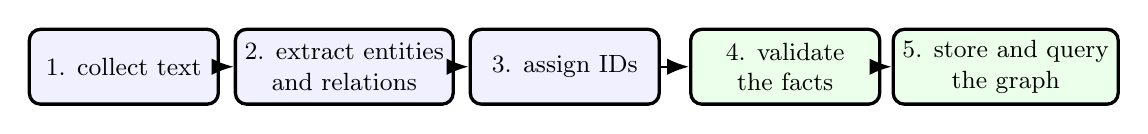
\begin{tikzpicture}[>=Latex, every node/.style={font=\small}]
  \node[stepbox] (t1) at (0,0) {1. collect text};
  \node[stepbox] (t2) at (2.8,0) {2. extract entities\\ and relations};
  \node[stepbox] (t3) at (5.6,0) {3. assign IDs};
  \node[stepbox2] (t4) at (8.4,0) {4. validate\\ the facts};
  \node[stepbox2] (t5) at (11.2,0) {5. store and query\\ the graph};
  \draw[flowarrow] (t1) -- (t2);
  \draw[flowarrow] (t2) -- (t3);
  \draw[flowarrow] (t3) -- (t4);
  \draw[flowarrow] (t4) -- (t5);
\end{tikzpicture}
\end{center}
\plainidea{Building a graph is a pipeline: extract, identify, validate, then store.}
\end{frame}

\begin{frame}{A Graph Needs Maintenance, Not Just Ingestion}
\keyquestion{What happens after the first version of the graph is built?}
\begin{center}
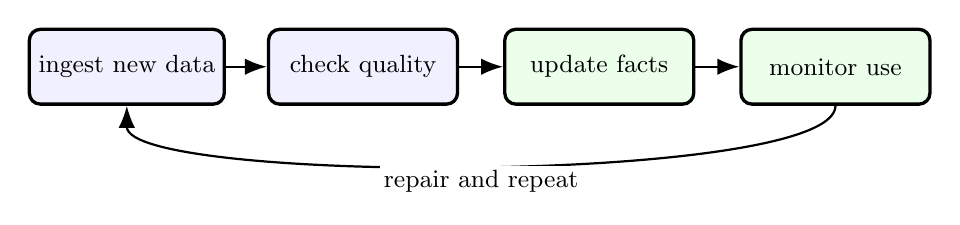
\begin{tikzpicture}[>=Latex, every node/.style={font=\small}]
  \node[stepbox] (a) at (0,0) {ingest new data};
  \node[stepbox] (b) at (3.0,0) {check quality};
  \node[stepbox2] (c) at (6.0,0) {update facts};
  \node[stepbox2] (d) at (9.0,0) {monitor use};
  \draw[flowarrow] (a) -- (b);
  \draw[flowarrow] (b) -- (c);
  \draw[flowarrow] (c) -- (d);
  \draw[flowarrow] (d.south) .. controls +(down:1.0cm) and +(down:1.0cm) .. node[relabel, below]{repair and repeat} (a.south);
\end{tikzpicture}
\end{center}
\plainidea{A real knowledge graph is a living system. It needs checking, updating, and repairing over time.}
\end{frame}

\begin{frame}{Why Knowledge Graphs Matter in Modern AI}
\keyquestion{Why are knowledge graphs still useful when we already have large language models?}
\begin{center}
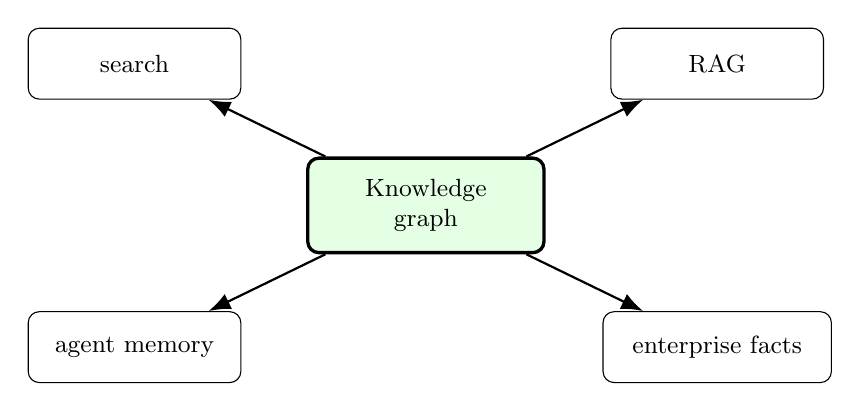
\begin{tikzpicture}[>=Latex, every node/.style={font=\small}]
  \node[entity2, minimum width=3.0cm, minimum height=1.2cm] (kg) at (4.2,0) {Knowledge\\ graph};
  \node[softbox, minimum width=2.7cm] (search) at (0.5,1.8) {search};
  \node[softbox, minimum width=2.7cm] (rag) at (7.9,1.8) {RAG};
  \node[softbox, minimum width=2.7cm] (memory) at (0.5,-1.8) {agent memory};
  \node[softbox, minimum width=2.9cm] (enterprise) at (7.9,-1.8) {enterprise facts};
  \draw[flowarrow] (kg) -- (search);
  \draw[flowarrow] (kg) -- (rag);
  \draw[flowarrow] (kg) -- (memory);
  \draw[flowarrow] (kg) -- (enterprise);
\end{tikzpicture}
\end{center}
\plainidea{LLMs are strong language models. Graphs give them explicit and grounded facts.}
\end{frame}

\begin{frame}{KG-to-Agent Context Pipeline}
\keyquestion{How does an agent turn a user question into grounded context from a graph?}
\begin{center}
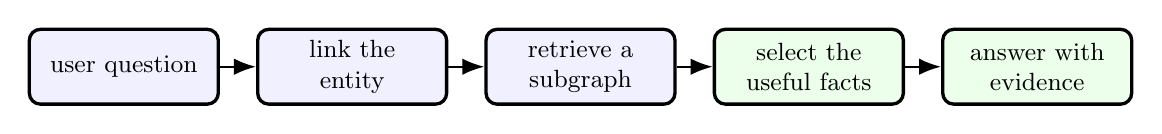
\begin{tikzpicture}[>=Latex, every node/.style={font=\small}]
  \node[stepbox] (q) at (0,0) {user question};
  \node[stepbox] (l) at (2.9,0) {link the\\ entity};
  \node[stepbox] (r) at (5.8,0) {retrieve a\\ subgraph};
  \node[stepbox2] (s) at (8.7,0) {select the\\ useful facts};
  \node[stepbox2] (a) at (11.6,0) {answer with\\ evidence};
  \draw[flowarrow] (q) -- (l);
  \draw[flowarrow] (l) -- (r);
  \draw[flowarrow] (r) -- (s);
  \draw[flowarrow] (s) -- (a);
\end{tikzpicture}
\end{center}
\plainidea{The agent should not answer first and search later. It should retrieve evidence first, then answer.}
\end{frame}

\begin{frame}{Do Not Send the Whole Graph}
\keyquestion{Why do we need to reduce the graph before giving context to an LLM?}
\begin{center}
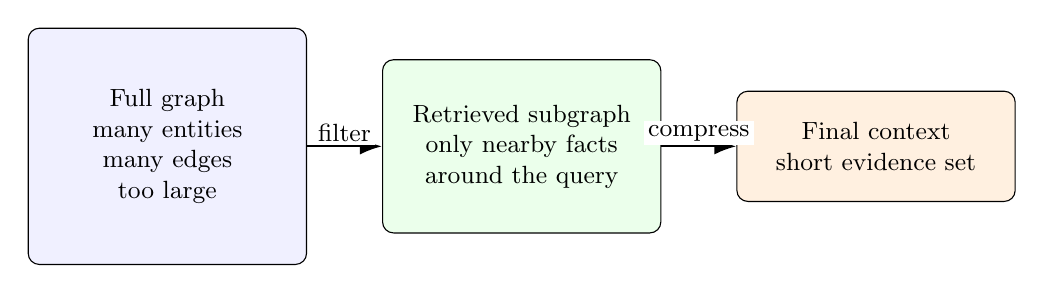
\begin{tikzpicture}[>=Latex, every node/.style={font=\small}]
  \node[draw, rounded corners, fill=blue!6, text width=3.3cm, minimum height=3.0cm, align=center] (full) at (0,0) {Full graph\\ many entities\\ many edges\\ too large};
  \node[draw, rounded corners, fill=green!8, text width=3.3cm, minimum height=2.2cm, align=center] (sub) at (4.5,0) {Retrieved subgraph\\ only nearby facts\\ around the query};
  \node[draw, rounded corners, fill=orange!12, text width=3.3cm, minimum height=1.4cm, align=center] (ctx) at (9.0,0) {Final context\\ short evidence set};
  \draw[flowarrow] (full) -- node[relabel, above]{filter} (sub);
  \draw[flowarrow] (sub) -- node[relabel, above]{compress} (ctx);
\end{tikzpicture}
\end{center}
\plainidea{A good system narrows the graph down to only the evidence that fits the question and the context budget.}
\end{frame}

\begin{frame}{Grounded Tool Use Needs Guardrails}
\keyquestion{How do we stop an agent from inventing graph facts that were never retrieved?}
\begin{center}
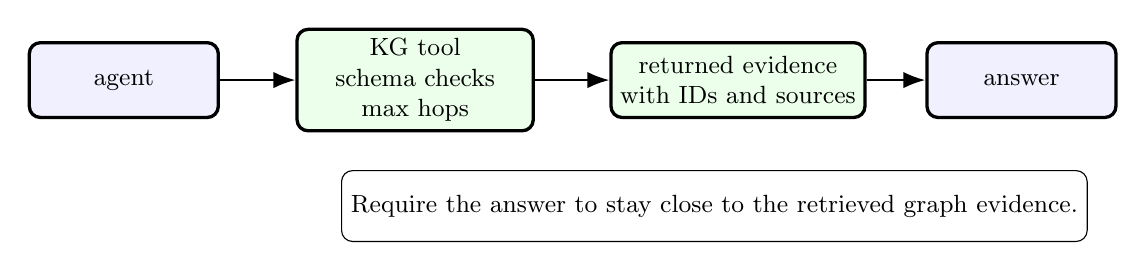
\begin{tikzpicture}[>=Latex, every node/.style={font=\small}]
  \node[stepbox] (agent) at (0,0) {agent};
  \node[stepbox2, minimum width=3.0cm] (tool) at (3.7,0) {KG tool\\ schema checks\\ max hops};
  \node[stepbox2, minimum width=3.0cm] (ev) at (7.8,0) {returned evidence\\ with IDs and sources};
  \node[stepbox] (ans) at (11.4,0) {answer};
  \draw[flowarrow] (agent) -- (tool);
  \draw[flowarrow] (tool) -- (ev);
  \draw[flowarrow] (ev) -- (ans);
  \node[softbox, minimum width=4.6cm] at (7.5,-1.6) {Require the answer to stay close to the retrieved graph evidence.};
\end{tikzpicture}
\end{center}
\plainidea{Guardrails keep the agent grounded in retrieved facts instead of imagined facts.}
\end{frame}

\begin{frame}{Campus Assistant Example}
\keyquestion{What could a small teaching assistant graph look like?}
\begin{center}
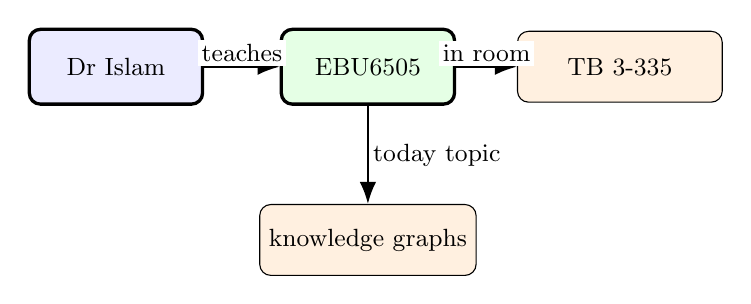
\begin{tikzpicture}[>=Latex, every node/.style={font=\small}]
  \node[entity2] (mod) at (3.4,0.8) {EBU6505};
  \node[entity] (teacher) at (0.2,0.8) {Dr Islam};
  \node[note] (room) at (6.6,0.8) {TB 3-335};
  \node[note] (topic) at (3.4,-1.4) {knowledge graphs};
  \draw[flowarrow] (teacher) -- node[relabel, above]{teaches} (mod);
  \draw[flowarrow] (mod) -- node[relabel, above]{in room} (room);
  \draw[flowarrow] (mod) -- node[relabel, right]{today topic} (topic);
\end{tikzpicture}
\end{center}
\begin{itemize}\small
  \item A student can ask: Who teaches EBU6505?
  \item A student can ask: Where is the class?
  \item A student can ask: What topic is today?
\end{itemize}
\plainidea{Even a small graph can support several useful questions when the entities and relations are clear.}
\end{frame}

\begin{frame}{Mini Design Exercise}
\keyquestion{If you built a graph for a campus assistant, which entities and relations would you include first?}
\begin{columns}[T,onlytextwidth]
  \begin{column}{0.48\textwidth}
    \begin{tcolorbox}[colback=questionbg,colframe=questionframe,boxrule=0.7pt,title=Possible entities]
    module, lecturer, room, student, deadline
    \end{tcolorbox}
    \begin{tcolorbox}[colback=plainbg,colframe=plainframe,boxrule=0.7pt,title=Possible relations]
    teaches, in room, has deadline, enrolled in
    \end{tcolorbox}
  \end{column}
  \begin{column}{0.48\textwidth}
    \begin{tcolorbox}[colback=notationbg,colframe=notationframe,boxrule=0.7pt,title=Task]
    Write:
    \begin{itemize}
      \item 4 entity types
      \item 4 relation types
      \item 2 example questions your graph should answer
    \end{itemize}
    \end{tcolorbox}
  \end{column}
\end{columns}
\plainidea{Design starts from the questions you want the graph to answer.}
\end{frame}

\begin{frame}{Transition to Day 4}
\keyquestion{Once the graph exists, how do search, RAG, and modern agents use it at run time?}
\begin{itemize}
  \item Today focused on the structure and maintenance of the graph.
  \item The next lecture focuses on using that graph inside modern AI pipelines.
  \item We will move from graph foundations to graph use in retrieval and reasoning.
\end{itemize}
\plainidea{Day 3 is about building the graph well. Day 4 is about using the graph well.}
\end{frame}

\begin{frame}{Key Takeaways}
\begin{itemize}
  \item A knowledge graph is a connected set of machine-usable facts.
  \item Graph paths support one-hop and multi-hop question answering.
  \item IDs, provenance, freshness, and entity resolution are essential, not optional.
  \item Modern AI systems use graphs as grounded evidence stores for retrieval and reasoning.
\end{itemize}
\plainidea{If the graph is clear and well maintained, it becomes a strong foundation for knowledge-based reasoning and RAG.}
\end{frame}

\begin{frame}{Further Study}
\begin{itemize}
  \item Read Poole Chapter 16 and revisit AIMA Chapter 10.
  \item Practice: Poole Ch.16, Exercises 16.2, 16.3, 16.4, 16.5, and 16.9.
  \item AIMA knowledge-representation exercise page: 3, 7, 8, 16, and 26.
  \item Focus on schema versus instance facts, connected triples, and what provenance adds to an answer.
\end{itemize}
\end{frame}

\end{document}
